\documentclass[11pt]{article}
\textheight 9in
\textwidth 6.5in
\oddsidemargin 0in
\topmargin 0in
\headheight 1in
\headsep 0in
\usepackage{color}
\usepackage{lastpage}
\usepackage{graphicx}
\usepackage{fancyhdr}
\pagestyle{fancy}
\cfoot{}
\rhead{\thepage\ of \pageref{LastPage}}
% \renewcommand{\headrulewidth}{0pt}
\usepackage[top = 4em, headsep=.2in]{geometry}
\usepackage{textcomp}
\usepackage{enumitem}

\begin{document}

\noindent{{\textbf{\large Spring 2020  \hfill Stat 305 (Section 4)
\hfill %Page \thepage   { of }  \pageref{lastpage}
Quiz 4}}

\vspace{2em}

\noindent\framebox(200, 50){\vspace{3em}\hspace{2em}\bf Name: \hspace{6cm}}

\bigskip

\noindent\emph{Total points for the exam is 50. Points for
individual questions are given at the beginning of each problem.
Show all your calculations clearly. Put final answers in the box at
the right (except for the diagrams!).}


\bigskip


%
\noindent \noindent {\bf 1.}\hfill[5+5+5+10=25 points] \\
%
\noindent B. Choi tested the stopping properties of various bike tires on various surfaces. For one thing, he tested both treaded and smooth tires on dry concrete. The lengths of skid marks produced in his study under these two conditions were as follows (in cm). Denote the true mean length of skid marks for treaded tires $\mu_1$ and the true mean length of skid marks for smooth tires $\mu_2$. 

\begin{center}
\begin{tabular}{|c|c|}
  \hline
  % after \\: \hline or \cline{col1-col2} \cline{col3-col4} ...
  Treaded & Smooth\\
  \hline
  365, 374, 376, 391, 401, 402 & 341, 348, 349, 355, 375, 391\\
   $\bar{x}_1 = 384.8333$ & $\bar{x}_2 = 359.8333$\\
   $s_1 = 15.38072$ & $s_2 = 19.16681$\\
  \hline
\end{tabular}
\end{center}




\begin{enumerate}
\item[(a)] Give a 95\% upper confidence bound for the mean length of skid marks for treaded tires in this study. (No need to simplify.)

\hfill \fbox{ \textcolor[rgb]{1.00,1.00,1.00}{{\LARGE
${\widehat{\widehat{\widehat \bigcap} }}$}} \hskip -0.4cm upper conf
bd = \hspace{8cm}}
%
%\hfill \fbox{ \textcolor[rgb]{1.00,1.00,1.00}{$\bigcap$} \hskip
%-0.4cm Equation 2: $\; \hat y =$ \hspace{10cm}}


\vskip 4.5cm

\item[(b)] Give a 90\% lower prediction bound for the length of skid mark in a single additional test for treaded tires in this study. (No need to simplify.)

\hfill \fbox{ \textcolor[rgb]{1.00,1.00,1.00}{{\LARGE
${\widehat{\widehat{\widehat \bigcap} }}$}} \hskip -0.4cm lower pred
bd = \hspace{8cm}}

\vskip 5cm

\item[(c)] Assuming the true standard deviations for treaded tires and smooth tires are equal ($\sigma_1 = \sigma_2$), give a 95\% two-sided confidence interval for the mean difference in lengths of skid marks for treaded tire and smooth tire (i.e. $\mu_1 - \mu_2$). (No need to simplify.)

\hfill \fbox{ \textcolor[rgb]{1.00,1.00,1.00}{{\LARGE
${\widehat{\widehat{\widehat \bigcap} }}$}} \hskip -0.4cm conf.
interval = \hspace{12cm}}

 \vskip 7cm

\item[(d)] Supposing the equal variance assumption in (c) still holds, use the hypothesis testing with p-value to assess the strength of evidence to support that
there is a mean difference in lengths of skid marks for treaded tire and smooth tire. (Show all the steps)

\end{enumerate}

\newpage

%--------------------------------

\noindent {\bf 2.}\hfill[9+1+5+5+5=25 points] \\
%
The data below were collected for studying the physical property of concrete made using burned clay aggregates. 10 batches of this kind of concrete are collected. The response
$y$ is compressive strength (in psi) and $x$ is splitting tensile strength (in psi).\\
%

\begin{tabular}{|r|c c c c c c c c c c|}
  \hline
  % after \\: \hline or \cline{col1-col2} \cline{col3-col4} ...
  $x$ & 207 & 233 & 254 & 328 & 325 & 302 & 258 & 335 & 315 & 302 \\
  \hline
  $y$ & 1420 & 1950 & 2230 & 3070 & 3060 & 3110 & 2650 & 3130 & 2960 & 2760 \\
  \hline
\end{tabular}
%
\vskip 0.5cm

\noindent Use the JMP output on page 6 answering the
following questions. \\ Note that $\bar x$ = 285.9, and
$\sum(x_i-\bar x)^2$= 17896.9.





\begin{enumerate}

\item[(a)] Use the hypothesis testing with $F$ statistic and the corresponding p-value to assess the strength of evidence to support that
the slope $\beta_1$ is different from 0. (Show all steps.)

\vskip 12cm

\item[(b)] Is the splitting tensile strength ($x$) a useful predictor for the compressive strength ($y$)? (Give a simple yes or no answer.)

\hfill \fbox{ \textcolor[rgb]{1.00,1.00,1.00}{{\LARGE
${\widehat{\widehat{\widehat \bigcap} }}$}} \hskip -0.4cm answer:\hspace{4cm}}

\clearpage
\item[(c)] Give a 95\% two-sided confidence interval for the expected change in compressive strength for a 1 unit
increase in splitting tensile strength. (No need to simplify.)

\hfill \fbox{ \textcolor[rgb]{1.00,1.00,1.00}{{\LARGE
${\widehat{\widehat{\widehat \bigcap} }}$}} \hskip -0.4cm conf.
interval = \hspace{10cm}}

 \vskip 6cm

\item[(c)] Give a 95\% lower confidence bound for the mean compressive strength when splitting tensile strength is 300 psi. (No need
to simplify.)

\hfill \fbox{ \textcolor[rgb]{1.00,1.00,1.00}{{\LARGE
${\widehat{\widehat{\widehat \bigcap} }}$}} \hskip -0.4cm lower conf
bd = \hspace{10cm}}

\vskip 6cm

\item[(d)] Give a 95\% two-sided prediction interval for the next compressive stength when the splitting tensile strength is 300 psi. (No
    need to simplify.)

\hfill \fbox{ \textcolor[rgb]{1.00,1.00,1.00}{{\LARGE
${\widehat{\widehat{\widehat \bigcap} }}$}} \hskip -0.4cm pred.
interval = \hspace{10cm}}

 \vskip 2.3cm

\end{enumerate}


\clearpage
\hspace{0pt}
\vfill

\centering
This page is intended to be blank.

\vfill

\hspace{0pt}
\clearpage



\section*{JMP Output}

% \subsection*{Fit 1}

% 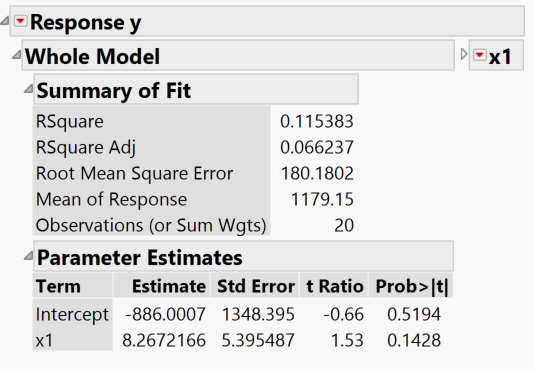
\includegraphics[width = 0.6\textwidth]{./q2x1.PNG}

% \subsection*{Fit 2}
\centering
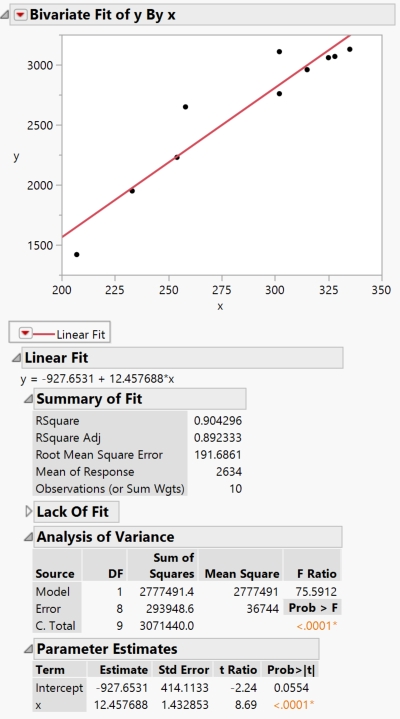
\includegraphics[width =0.8\textwidth]{./JMPoutput.PNG}
%
\label{lastpage}


\end{document}
